\begin{mdframed}
    \textbf{La extensión máxima para esta sección es de 6 páginas.}
\end{mdframed}


En esta sección, los resultados obtenidos, como las gráficas o tablas, deben estar respaldados por los datos generados durante la ejecución de sus programas. Es fundamental que, junto con el informe, se adjunten los archivos que contienen dichos datos para permitir su verificación. Además, se debe permitir y especficiar como obtener esos archivos desde una ejecución en otro computador (otra infraestructura para hacer lso experimentos).

\textbf{Es necesario automatizar la generación de las gráficas}, ya que es imprescindible que se pueda confirmar que las visualizaciones presentadas son producto de los datos generados por sus algoritmos.

Agregue gráficas que muestren los resultados de sus experimentos. La cantidad de páginas es limitada, por lo tanto escoja las gráficas más representativas y que muestren de manera clara los resultados obtenidos. Esta elección es parte de lo que se evaluara en la sección de presentación de resultados. Referencie las figuras en el texto, describa lo que se observa en ellas y por qué son relevantes.




\begin{figure}[H]
    \centering
    \begin{minipage}[t]{0.5\textwidth}
        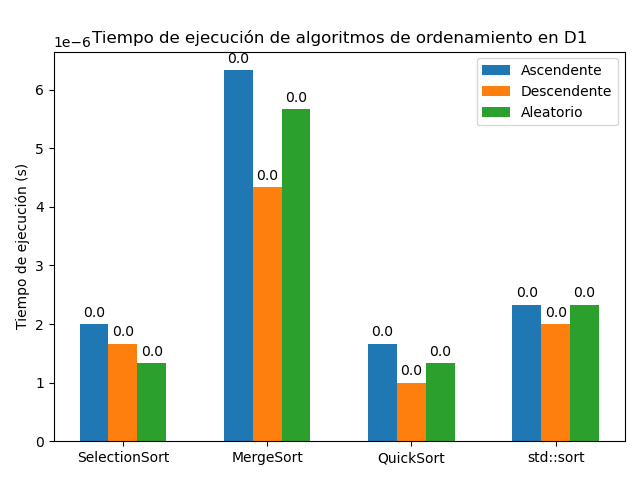
\includegraphics[width=\textwidth]{../code/sorting/data/plots/10_D1.png}
    \end{minipage}%
    \begin{minipage}[t]{0.5\textwidth}
        \includegraphics[width=\textwidth]{../code/sorting/data/plots/10_D2.png}
     \end{minipage}%
    \caption{Gráficos de tiempo de ejecución cuando N = 10, para los dominios D1 y D7 respectivamente.}
    \label{fig:sortingN10}
\end{figure}

\begin{figure}[H]
    \centering
    \begin{minipage}[t]{0.5\textwidth}
        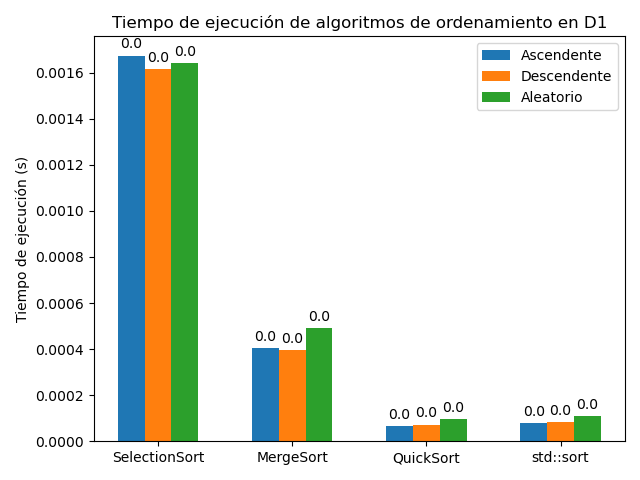
\includegraphics[width=\textwidth]{../code/sorting/data/plots/1000_D1.png}
    \end{minipage}%
    \begin{minipage}[t]{0.5\textwidth}
        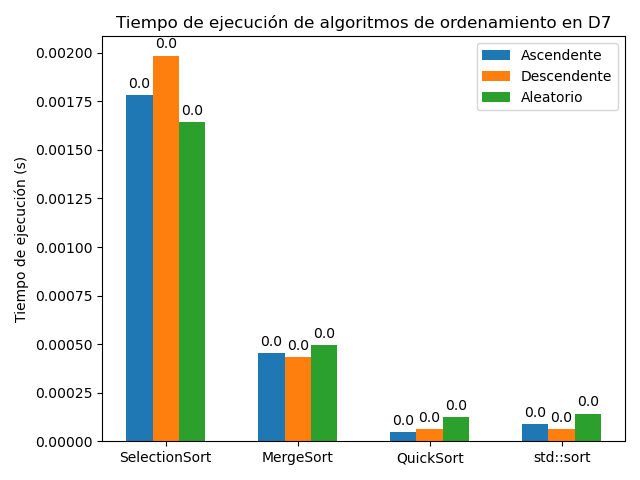
\includegraphics[width=\textwidth]{../code/sorting/data/plots/1000_D7.png}
     \end{minipage}%
    \caption{Gráficos de tiempo de ejecución cuando N = 1000, para los dominios D1 y D7 respectivamente.}
    \label{fig:sortingN1000}
\end{figure}


\begin{figure}[H]
    \centering
    \begin{minipage}[t]{0.5\textwidth}
        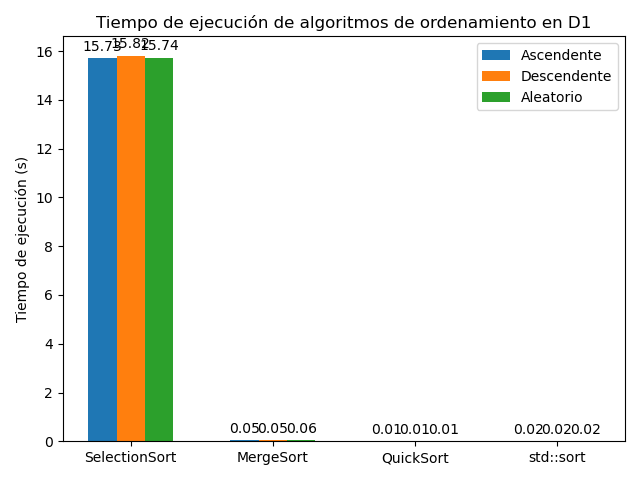
\includegraphics[width=\textwidth]{../code/sorting/data/plots/100000_D1.png}
    \end{minipage}%
    \begin{minipage}[t]{0.5\textwidth}
        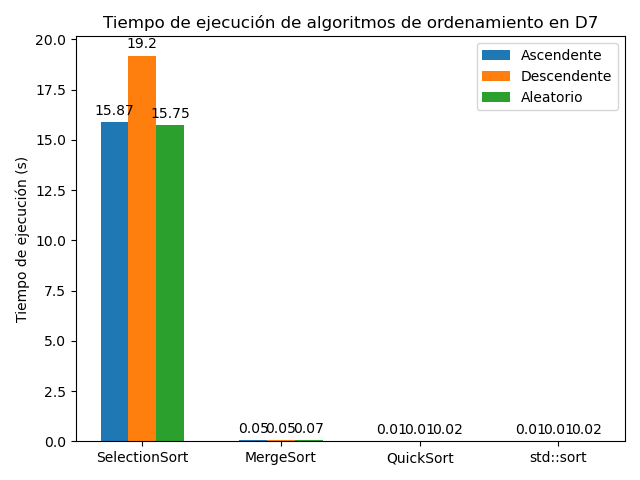
\includegraphics[width=\textwidth]{../code/sorting/data/plots/100000_D7.png}
     \end{minipage}%
    \caption{Gráficos de tiempo de ejecución cuando N = 100000, para los dominios D1 y D7 respectivamente.}
    \label{fig:sortingN100000}
\end{figure}

\begin{figure}[H]
    \centering
    \begin{minipage}[t]{0.5\textwidth}
        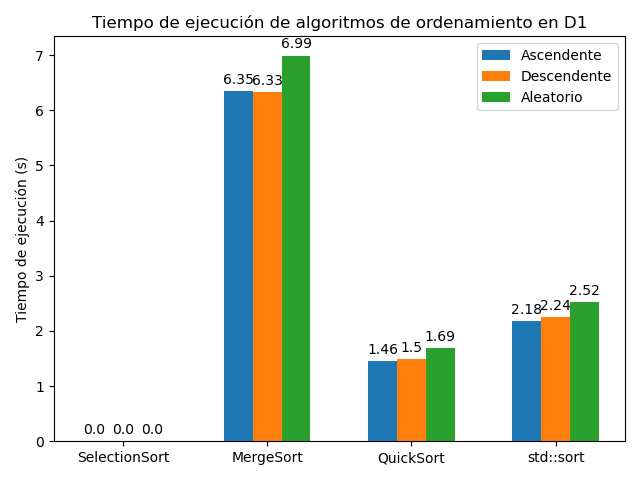
\includegraphics[width=\textwidth]{../code/sorting/data/plots/10000000_D1.png}
    \end{minipage}%
    \begin{minipage}[t]{0.5\textwidth}
        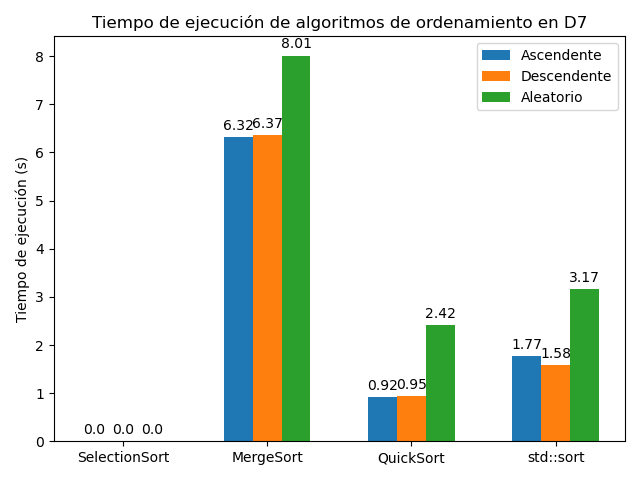
\includegraphics[width=\textwidth]{../code/sorting/data/plots/10000000_D7.png}
     \end{minipage}%
    \caption{Gráficos de tiempo de ejecución cuando N = 10000000, para los dominios D1 y D7 respectivamente.}
    \label{fig:sortingN10000000}
\end{figure}

Para los algoritmos de ordenamiento, se puede notar que para N = 10, los algoritmos corren casi al instante (por un bug, sale en segundos cada barrita a la izquierda, pero en realidad el tiempo de ejecución es chico al punto de expresarse en notación científica en las mediciones). SelectionSort saca tiempo de ejecución comparable con QuickSort y std::sort. En cambio, el más lento en este caso resulta ser MergeSort, pese a su complejidad $O(nlog(n))$; esto puede deberse por detalles en la implementación (recordar que lo implementé yo), o bien por overhead en la recursión.
\newline \newline
Para N = 1000, el tiempo de ejecución de SelectionSort ya se empieza a disparar comparado con los otros tres algoritmos de ordenamiento, aunque bien su tiempo de ejecución sigue siendo bastante rápido (menos de 2 centésimas de segundo). Esto es reflejo de su conocida complejidad temporal $O(n^2)$. En cambio, los otros tres algoritmos se benefician altamente de sus complejidades $O(nlogn)$, estando significativamente por delante de SelectionSort. No hay cambios significativos según la distribución de los elementos de la entrada.
\newline \newline
Para N = 100000, se repite lo antes visto para N = 1000, pero se acentúa aún más la diferencia de tiempo de ejecución de SelectionSort comparados con los otros algoritmos; llega a tardarse alrededor de 16 segundos por arreglo, mientras que el siguiente peor algoritmo en este sentido es MergeSort con tan solo 5 centésimas de segundo.
\newline \newline
Para N = 10000000, se decidió derechamente omitir el SelectionSort, ya que al intentar correrlo con arreglos de este tamaño, legítimamente se demoraba demasiado, y se puede estimar a partir de los gráficos anteriores que iba a tardar varios minutos sólo para terminar de ordenar un arreglo de este tamaño.

Dicho esto, se puede observar un fenómeno interesante con los otros 3 algoritmos; sus tiempos de ejecución aumentan significativamente con los arreglos con elementos aleatorios en D7 (particularmente QuickSort).
\newline
\begin{figure}[H]
    \centering
    \begin{minipage}[t]{0.5\textwidth}
        \includegraphics[width=\textwidth]{../matrix_multiplication/data/plots/16_D1.png}
    \end{minipage}%
    \begin{minipage}[t]{0.5\textwidth}
        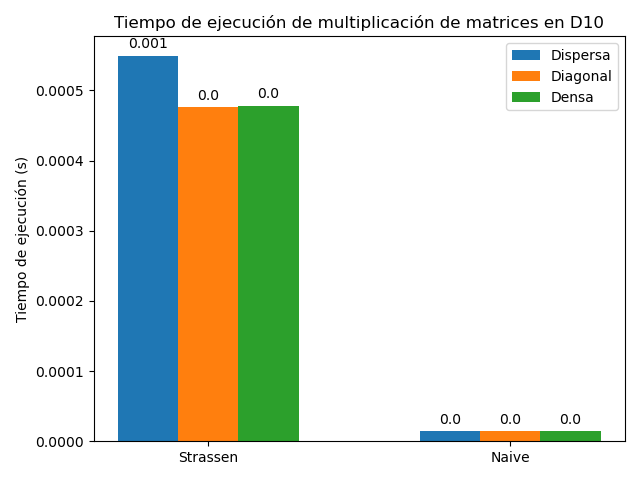
\includegraphics[width=\textwidth]{../matrix_multiplication/data/plots/16_D10.png}
     \end{minipage}%
    \caption{Gráficos de tiempo de ejecución de multiplicación de matrices cuando N = 16, para los dominios D1 y D10 respectivamente.}
    \label{fig:matrixN2}
\end{figure}

\begin{figure}[H]
    \centering
    \begin{minipage}[t]{0.5\textwidth}
        \includegraphics[width=\textwidth]{../matrix_multiplication/data/plots/64_D1.png}
    \end{minipage}%
    \begin{minipage}[t]{0.5\textwidth}
        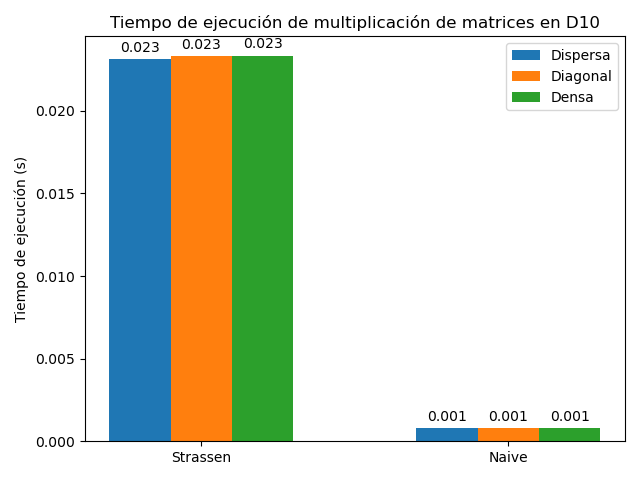
\includegraphics[width=\textwidth]{../matrix_multiplication/data/plots/64_D10.png}
     \end{minipage}%
    \caption{Gráficos de tiempo de ejecución de multiplicación de matrices cuando N = 64, para los dominios D1 y D10 respectivamente.}
    \label{fig:matrixN2}
\end{figure}

\begin{figure}[H]
    \centering
    \begin{minipage}[t]{0.5\textwidth}
        \includegraphics[width=\textwidth]{../matrix_multiplication/data/plots/256_D1.png}
    \end{minipage}%
    \begin{minipage}[t]{0.5\textwidth}
        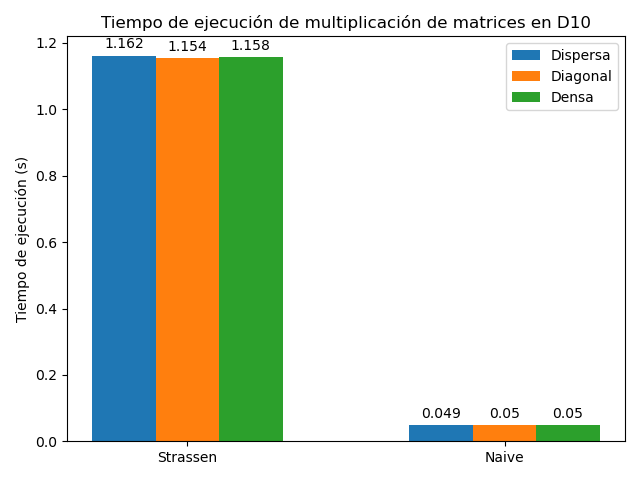
\includegraphics[width=\textwidth]{../matrix_multiplication/data/plots/256_D10.png}
     \end{minipage}%
    \caption{Gráficos de tiempo de ejecución de multiplicación de matrices cuando N = 256, para los dominios D1 y D10 respectivamente.}
    \label{fig:matrixN2}
\end{figure}

\begin{figure}[H]
    \centering
    \begin{minipage}[t]{0.5\textwidth}
        \includegraphics[width=\textwidth]{../matrix_multiplication/data/plots/1024_D1.png}
    \end{minipage}%
    \begin{minipage}[t]{0.5\textwidth}
        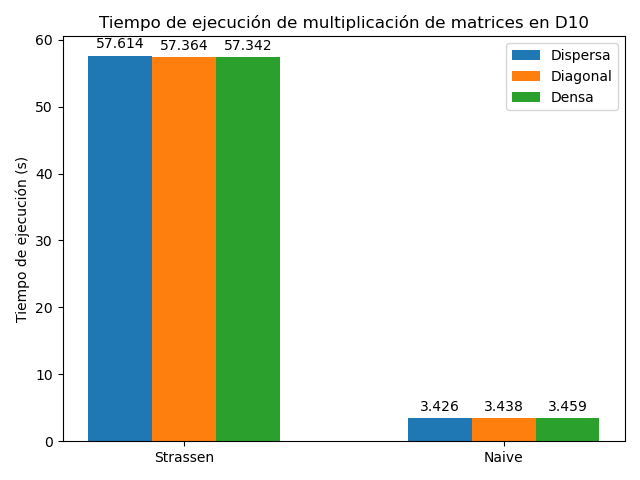
\includegraphics[width=\textwidth]{../matrix_multiplication/data/plots/1024_D10.png}
     \end{minipage}%
    \caption{Gráficos de tiempo de ejecución de multiplicación de matrices cuando N = 256, para los dominios D1 y D10 respectivamente.}
    \label{fig:matrixN2}
\end{figure}

En una sorpresa total, Strassen es bastante más lento que Naive para prácticamente todos los casos. Si bien Strassen teóricamente tiene una complejidad temporal de aproximadamente $O(n^{2,8})$ versus la de Naive, $O(n^3)$, lo más probable es que la cantidad de recursiones y arreglos auxiliares que se terminan creando generen una cantidad de overhead que elimina cualquier beneficio que el algoritmo podría haber tenido para estos casos; se necesitaría un valor de N muy, muy grande para que recién ahí empezara a alcanzarle al Naive en tiempo de ejecución. No obstante, tal valor necesariamente existe, pero los tamaños de las matrices no alcanzan a tal valor; no se observa una diferencia decreciente por los casos vistos.


\begin{mdframed}
    Recuerde que es imprescindible que se pueda replicar la generación de las gráficas, por lo que usted debe referir a las figuras generadas en `code/matrix\_multiplication/data/plots/` y `code/sorting/data/plots/`.
\end{mdframed}
